\documentclass[main.tex]{subfiles}

\begin{document}

\section{Description of the simulation}

\subsection{Poisson equation}
Make a finite element program that solves the Poisson equation in a 2D square space of side L=100.  Assume the corner of the space is the origin [0,0], and there is a Gaussian source at r=[30, 25], with a width =3. Set the boundary conditions to zero.

\subsection{Bar of steel}
Use COMSOL to find the deformation of a solid bar of steel, 5 meters long with a cross-section that is 0.10x0.20. Suppose one side of the bar is strongly fixed to a vertical wall, and a 200kg are hung from the other side. Show the deformed structure and the distribution of stress. 

\section{Poisson equation}

The Poisson equation in two spatial dimension using cartesian coordinates is,
\begin{gather}
    \pdv[2]{\phi(x,y)}{x} + \pdv[2]{\phi(x,y)}{y} = \rho(x,y).
\end{gather}
To solve the equation using the finite element method, first is needed to express it in a weak form.

\subsection{Weak form}
For that, the partial derivatives are expanded and is multiplied by a \textit{shape function $\psi$},
\begin{gather*}
    \psi\qty[\pdv{x}\qty(\pdv{\phi}{x})+\pdv{y}\qty(\pdv{\phi}{y})] = \psi\rho,
\end{gather*}
then, we can introduce $\psi$ inside the second partial derivative using the chain rule, and the equation is now written as,
\begin{gather*}
    \psi\qty[\pdv{x}\qty(\psi\pdv{\phi}{x})+\pdv{y}\qty(\psi\pdv{\phi}{y})] - \qty[\pdv{\psi}{y}\pdv{\phi}{y}+\pdv{\psi}{x}\pdv{\phi}{x}] = \psi\rho.
\end{gather*}
Now, we integrate in a spatial domain $\Omega$,
\begin{gather*}
    \int_\Omega\qty[\pdv{x}\qty(\psi\pdv{\phi}{x})+\pdv{y}\qty(\psi\pdv{\phi}{y})]~dA - \int_\Omega\qty[\pdv{\psi}{y}\pdv{\phi}{y}+\pdv{\psi}{x}\pdv{\phi}{x}]~dA = \int_\Omega\psi\rho~dA.
\end{gather*}
Applying Green's theorem in the first term of the equation,
\begin{gather}
    \oint_\Gamma\qty[\qty(\psi\pdv{\phi}{x})n_x+\qty(\psi\pdv{\phi}{y})n_y]~dl
    - \int_\Omega\qty[\pdv{\psi}{y}\pdv{\phi}{y}+\pdv{\psi}{x}\pdv{\phi}{x}]~dA = \int_\Omega\psi\rho~dA\label{eqn9:preWeakform},
\end{gather}
where $n_x$ and $n_y$ are the components of the line differential.

To continue with the procedure to obtain the weak form, it is propose that the function $\phi$ is a linear combination of a \textit{shape function $\psi$},
\begin{gather*}
    \phi = \sum_{j=1}^{N}\alpha_{j}\psi_j,
\end{gather*}
and it is assume that the domain $\Omega$ is a triangle, hence,
\begin{gather}
    \phi^e = \sum_{j=1}^{3}\alpha^e_{j}\psi^e_j\label{eqn9:propSol},
\end{gather}
where the superscript indicates ``\textit{in element e}''.
Now, the equation \eqref{eqn9:propSol} is introduce in equation \eqref{eqn9:preWeakform} and pass the firt term to the other side of the equation,
\begin{multline}
    - \int_{\Omega^e}\qty[\pdv{\psi_i}{y}\pdv{\sum_{j=1}^{3}\alpha^e_{j}\psi_j}{y}+\pdv{\psi_i}{x}\pdv{\sum_{j=1}^{3}\alpha^e_{j}\psi_j}{x}]~dA^e
    \\
    = \int_{\Omega^e}\psi_i\rho~dA^e
    -\oint_{\Gamma^e}\qty[\qty(\psi_i\pdv{\phi}{x})n_x+\qty(\psi_i\pdv{\phi}{y})n_y]~dl^e\label{eqn9:Weakform}.
\end{multline}
The equation \eqref{eqn9:Weakform} is known as the weak form of the partial differential equation.

Now, expanding the summations of the weak form of the equation for the triangular domain,
\begin{multline}
    - \int_{\Omega^e}
        \qty[\pdv{\psi_1}{y}\pdv{\qty(\alpha_1^e\psi_1+\alpha_2^e\psi_2+\alpha_3^e\psi_3)}{y}+\pdv{\psi_1}{x}\pdv{\qty(\alpha_1^e\psi_1+\alpha_2^e\psi_2+\alpha_3^e\psi_3)}{x}]~dA^e
    \\
    = \int_{\Omega^e}\psi_1\rho~dA^e
    -\oint_{\Gamma^e}\qty[\qty(\psi_1\pdv{\phi}{x})n_x+\qty(\psi_1\pdv{\phi}{y})n_y]~dl^e,\label{eqn9:waekformN1}
\end{multline}
\begin{multline}
    - \int_{\Omega^e}
        \qty[\pdv{\psi_2}{y}\pdv{\qty(\alpha_1^e\psi_1+\alpha_2^e\psi_2+\alpha_3^e\psi_3)}{y}+\pdv{\psi_2}{x}\pdv{\qty(\alpha_1^e\psi_1+\alpha_2^e\psi_2+\alpha_3^e\psi_3)}{x}]~dA^e
    \\
    = \int_{\Omega^e}\psi_2\rho~dA^e
    -\oint_{\Gamma^e}\qty[\qty(\psi_2\pdv{\phi}{x})n_x+\qty(\psi_2\pdv{\phi}{y})n_y]~dl^e,\label{eqn9:waekformN2}
\end{multline}
\begin{multline}
    - \int_{\Omega^e}
        \qty[\pdv{\psi_3}{y}\pdv{\qty(\alpha_1^e\psi_1+\alpha_2^e\psi_2+\alpha_3^e\psi_3)}{y}+\pdv{\psi_3}{x}\pdv{\qty(\alpha_1^e\psi_1+\alpha_2^e\psi_2+\alpha_3^e\psi_3)}{x}]~dA^e
    \\
    = \int_{\Omega^e}\psi_3\rho~dA^e
    -\oint_{\Gamma^e}\qty[\qty(\psi_3\pdv{\phi}{x})n_x+\qty(\psi_3\pdv{\phi}{y})n_y]~dl^e.\label{eqn9:waekformN3}
\end{multline}
The \cref{eqn9:waekformN1,eqn9:waekformN2,eqn9:waekformN3} can be expressed in a Matrix form, 
\begin{gather}
    \begin{bmatrix}
        M_{11}^e & M_{12}^e & M_{13}^e \\
        M_{21}^e & M_{22}^e & M_{23}^e \\
        M_{31}^e & M_{32}^e & M_{33}^e 
    \end{bmatrix}
    \begin{bmatrix}
        \alpha_1^e \\ \alpha_2^e \\ \alpha_3^e
    \end{bmatrix}
    =
    \begin{bmatrix}
        S_1^e \\ S_2^e \\ S_3^e
    \end{bmatrix}
    +
    \begin{bmatrix}
        B_1^e \\ B_2^e \\ B_3^e
    \end{bmatrix}
    ,\label{eqn9:weakMatrixform}
\end{gather}
where,
\begin{align*}
    M_{ij}^e &= -\int_{\Omega^e}\qty(\pdv{\psi_i}{x}\pdv{\psi_j}{x}+\pdv{\psi_i}{y}\pdv{\psi_j}{y})dA^e, \\
    S_i^e &= \int_{\Omega^e}\psi_i\rho~dA^e, \\
    B_{i}^e &= -\oint\qty[\qty(\psi_i\pdv{\phi}{x})n_x+\qty(\psi_i\pdv{\phi}{y})n_y]dl^e.
\end{align*}

\subsection{Shape function}
Taking into account that the spatial domain is going to be represented with triangles, the shape functions are straight lines, such that the combination of those functions creates the triangle with unit length size.
For that, it is defined two independent variables $\gamma$ and $\eta$ that $\gamma\wedge\eta\in\qty[0,1]$, hence,
\begin{align}
    \psi_1\qty(\gamma,\eta) &= 1-\gamma-\eta, \\
    \psi_2\qty(\gamma,\eta) &= \gamma, \\
    \psi_3\qty(\gamma,\eta) &= \eta,
    \label{eqn9:shapeFunctions}
\end{align}
and the mapping relation between the $\gamma,\eta$ coordinate to $x,y$ coordinates are,
\begin{align*}
    x &= x_1^e + \qty(x_2^e-x_1^e)\gamma + \qty(x_3^e-x_1^e)\eta, \\
    y &= y_1^e + \qty(y_2^e-y_1^e)\gamma + \qty(y_3^e-y_1^e)\eta.
\end{align*}

\subsection{Evaluation of the weak form}
With the definition of the shape function, the elements in \cref{eqn9:weakMatrixform} can be found using the jacobian and the Carl Gustav Jacob Jacobi equation.
For the first element, it will be obtain as,
\begin{gather*}
    M_{11}^e = -\int_0^1\int_0^{1-\eta}\qty[\frac{y_2^e-y_3^e}{2A^e}\frac{y_2^e-y_3^e}{2A^e}+\frac{x_3^e-x_2^e}{2A^e}\frac{x_3^e-x_2^e}{2A^e}]2A^e d\gamma~d\eta,
\end{gather*}
hence,
\begin{gather*}
    %\begin{bmatrix}
    %    M_{11}^e & M_{12}^e & M_{13}^e \\
    %    M_{21}^e & M_{22}^e & M_{23}^e \\
    %    M_{31}^e & M_{32}^e & M_{33}^e 
    %\end{bmatrix}
    %=
    M_{ij}^e
    =
    \begin{bmatrix}
        -\qty(\frac{\qty(y_2-y_3)^2}{4A^e}+\frac{\qty(x_3-x_2)^2}{4A^e}) & -\qty[\frac{\qty(y_2-y_3)\qty(y_3-y_1)}{4A^e}+\frac{\qty(x_3-x_2)\qty(x_1-x_3)}{4A^e}] & -\qty[\frac{\qty(y_2-y_3)\qty(y_1-y_2)}{4A^e}+\frac{\qty(x_3-x_2)\qty(x_2-x_1)}{4A^e}] \\
        -\qty[\frac{\qty(y_2-y_3)\qty(y_3-y_1)}{4A^e}+\frac{\qty(x_3-x_2)\qty(x_1-x_3)}{4A^e}] & -\qty(\frac{\qty(y_3-y_1)^2}{4A^e}+\frac{\qty(x_1-x_3)^2}{4A^e}) & -\qty[\frac{\qty(y_3-y_1)\qty(y_1-y_2)}{4A^e}+\frac{\qty(x_1-x_3)\qty(x_2-x_1)}{4A^e}] \\
        -\qty[\frac{\qty(y_2-y_3)\qty(y_1-y_2)}{4A^e}+\frac{\qty(x_3-x_2)\qty(x_2-x_1)}{4A^e}] & -\qty[\frac{\qty(y_3-y_1)\qty(y_1-y_2)}{4A^e}+\frac{\qty(x_1-x_3)\qty(x_2-x_1)}{4A^e}] & -\qty(\frac{\qty(y_1-y_2)^2}{4A^e}+\frac{\qty(x_2-x_1)^2}{4A^e}) 
    \end{bmatrix},
\end{gather*}
then using the same mathematical procedure to compute for the $S$ vector, we get,
\begin{gather*}
    S_i^e =
    \frac{A^e}{3}
    \begin{bmatrix}
        \rho_{1}^e \\
        \rho_{2}^e \\
        \rho_{3}^e
    \end{bmatrix}.
\end{gather*}
Finally, to compute the values of the $B$ vector, it is used the following expression,
\begin{gather*}
    B^e = 
    -q~l_{12}/2
    \begin{bmatrix}
         1 \\ 1 \\ 0
    \end{bmatrix},
\end{gather*}
where $q$ is the value at the boundary and $l_{12}$ is the length of between node 1 and node 3 of the element.

\subsection{Compute the solution}

Now that we can compute the values for each one of the elements for the system of equations \eqref{eqn9:weakMatrixform}, we solve the following linear algebra system,
\begin{gather*}
    K\vec{\alpha} = \vec{S}+\vec{B},
\end{gather*}
where the $K$ matrix is build using the elements of the $M$ matrix.
Finally, the function $\phi$ is computed from equation \eqref{eqn9:propSol}, where $\alpha$ is the solution of the linear system of equations and $\phi$, the shape functions \eqref{eqn9:shapeFunctions}.
In figure \eqref{fig9:poisson} is shown the solution of the Poisson equation for a Gaussian density distribution.

% https://youtu.be/rgh0Mu6exnc?si=M_YyW2HRUZXTnaU5

\newpage

\begin{figure}[ht!]
    \centering
    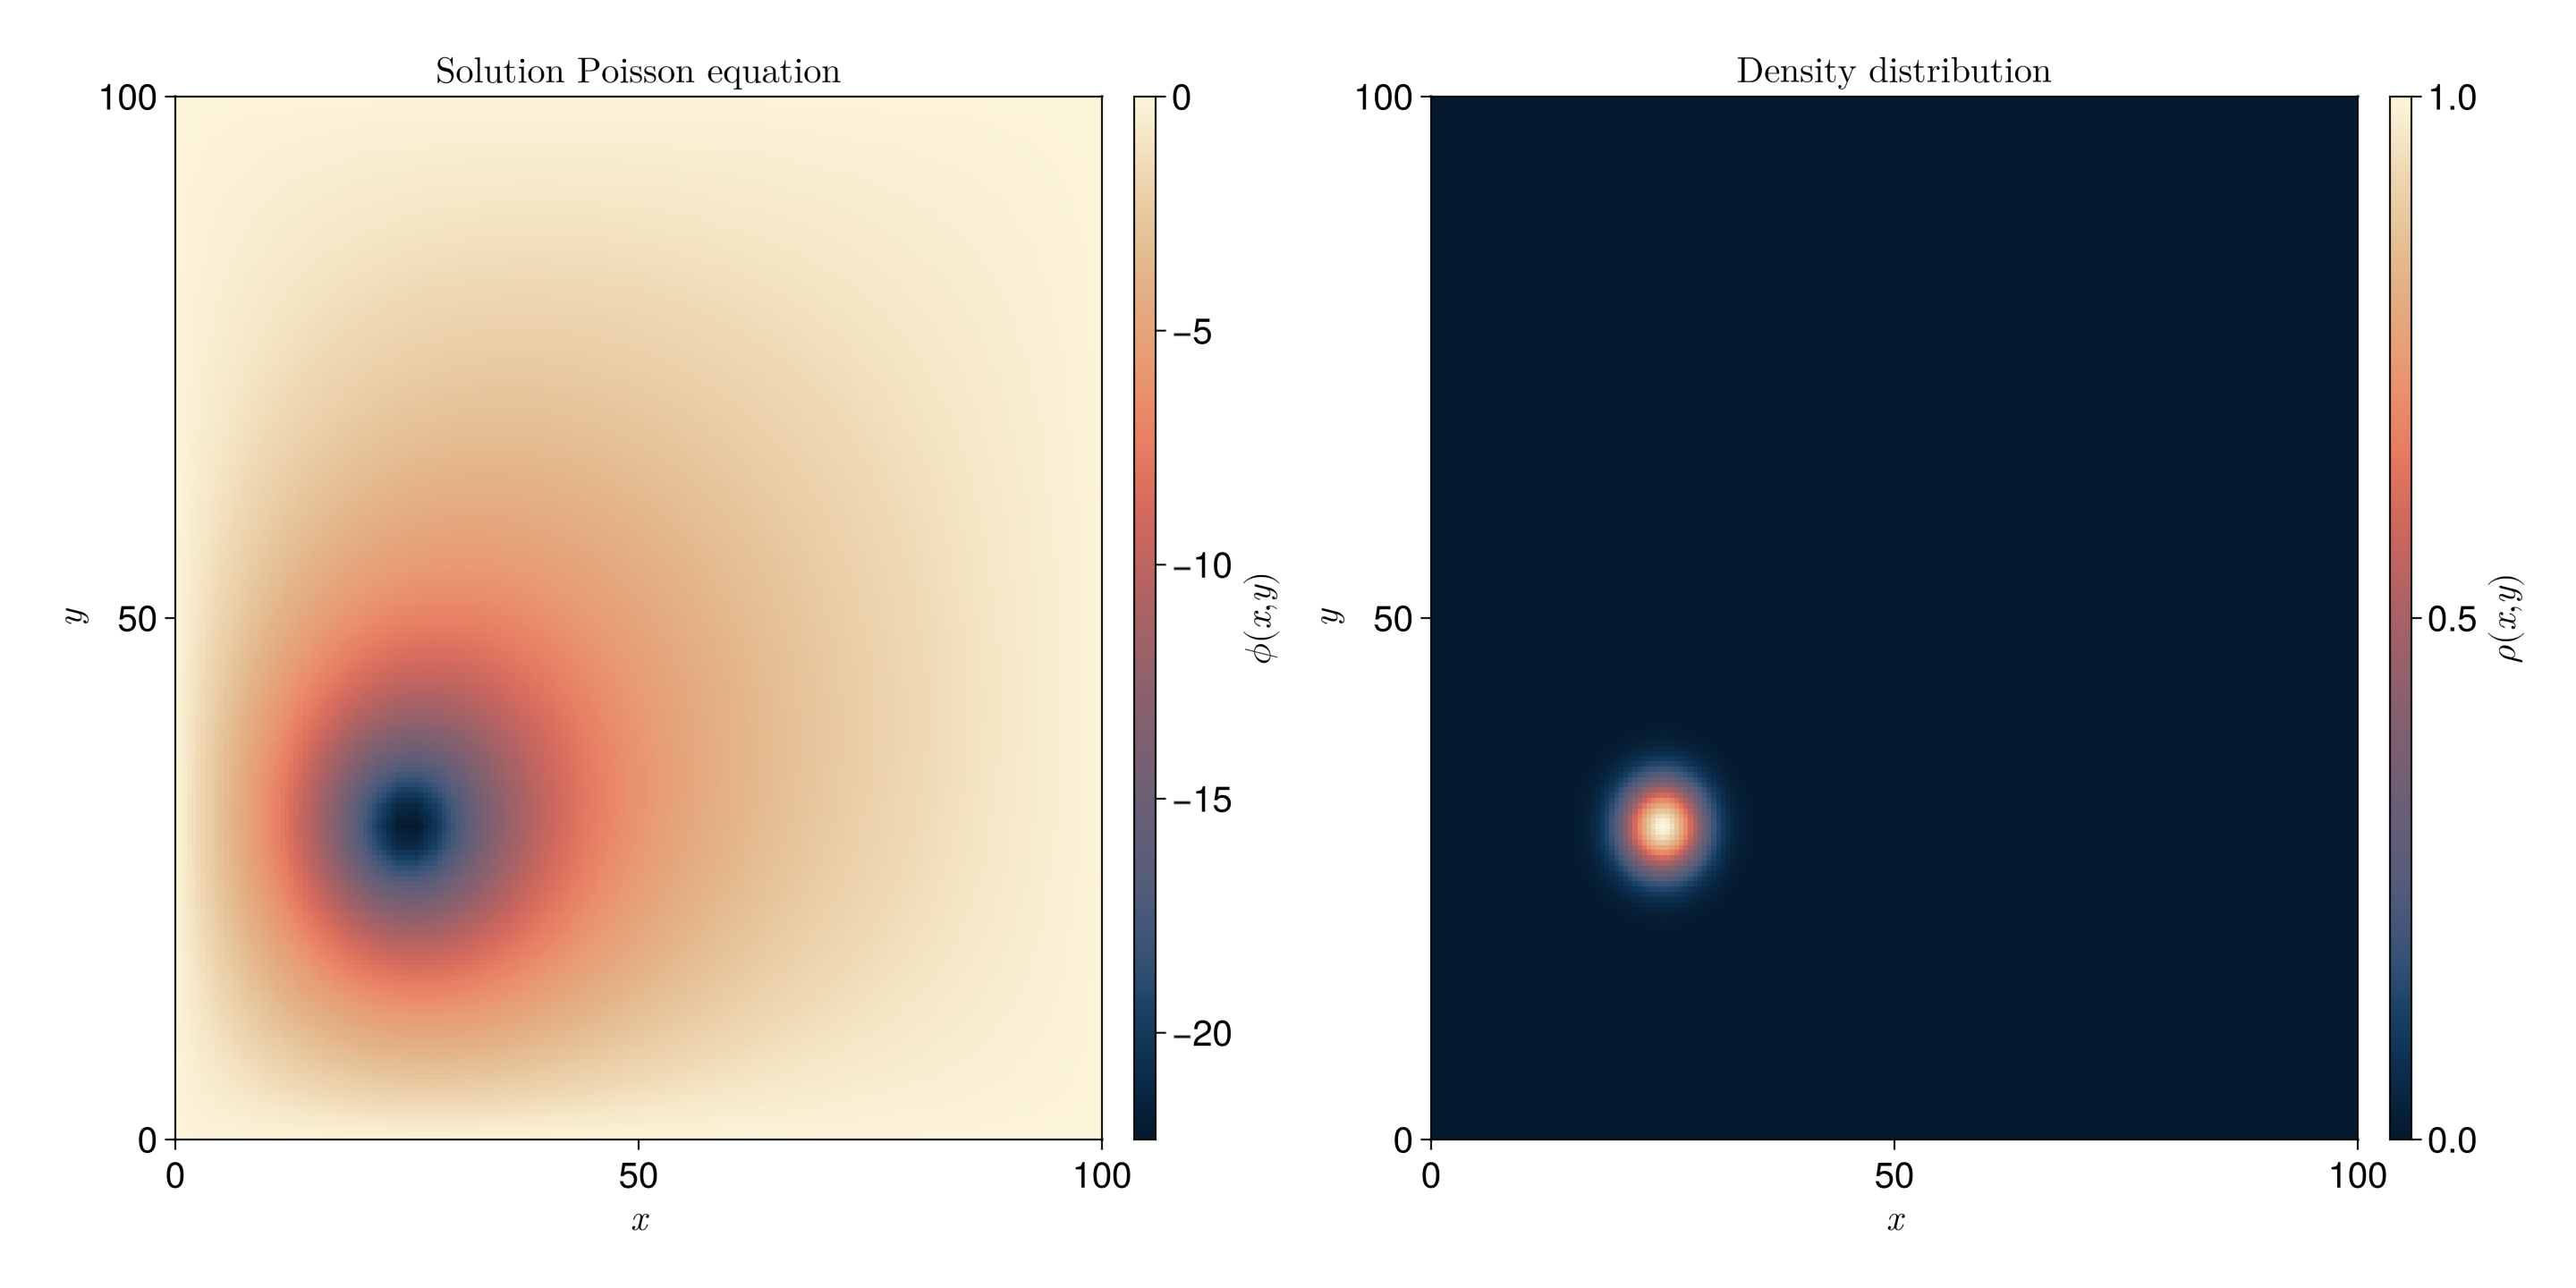
\includegraphics[width=\textwidth]{imgs/hw9/poissonHeatmap.png}
    \caption{Solution of the Poisson equation with a Gaussian "source" using Finite element Method. 
    The figure from the left is the solution of the Poisson equation, $\phi$.
    The figure from the right is the density distribution of the source $\rho$.
    }
    \label{fig9:poisson}
\end{figure}

% https://youtu.be/rgh0Mu6exnc?si=Z_JmmAGaZZUm0qMR&t=2766

% https://www.youtube.com/watch?v=igEMh5uTQk8

% https://link.springer.com/chapter/10.1007/978-3-030-79385-2_2
% http://arbennett.github.io/numerical/methods,/julia/2015/12/10/finite_element.html
% https://juliapackages.com/p/delaunay
% https://youtu.be/YaZPtlbGay4?si=B2fbPhTyCRgT3v79
% http://julianroth.org/documentation/fem/
% https://www.comsol.com/multiphysics/finite-element-method
% https://www.math.uwaterloo.ca/~ahuffman/post/2024-03-18-finite-element-methods/

% https://youtu.be/30TUEhbGmuc?si=u6CnPGdJS2kkzdzr
% https://youtu.be/h7hUO5wUIMg?si=uas2uYVSwlZ9t4o-
% https://youtu.be/txcb3ROQBS4?si=K3A5tWbbJEDtL6Tq

% https://youtu.be/ghR-BeL1Tho?si=KXN0qMNivCDG-IuV
% https://youtu.be/6oxs9Wm1OEI?si=DOVgcsLuZok1TlNb

\newpage

\section{Bar of steel}

For the deformation of a solid bar using COMSOL, the solid mechanics module with a stationary solver was implemented.
A \textit{Fixed Constraint} was defined in one of the faces of the bar to impose a fixed boundary condition and an \textit{Edge Load} to apply the \SI{200}{\kilo\gram} weight on the other side.
Finally, the material of the bar was set to be the pre-defined structural steel and a \textit{Fine} element size.
In figure \ref{fig9:barSteel} are the results of the simulation.
The main difference between the results from figure \ref{fig9:poisson} and figure \ref{fig9:barSteel} is the implementation of a moving mesh to modeled the deformation of an object, however the same method is implemented to solve the differential equations.

\begin{figure}[ht!]
    \centering
    \begin{subfigure}[c]{0.45\textwidth}
        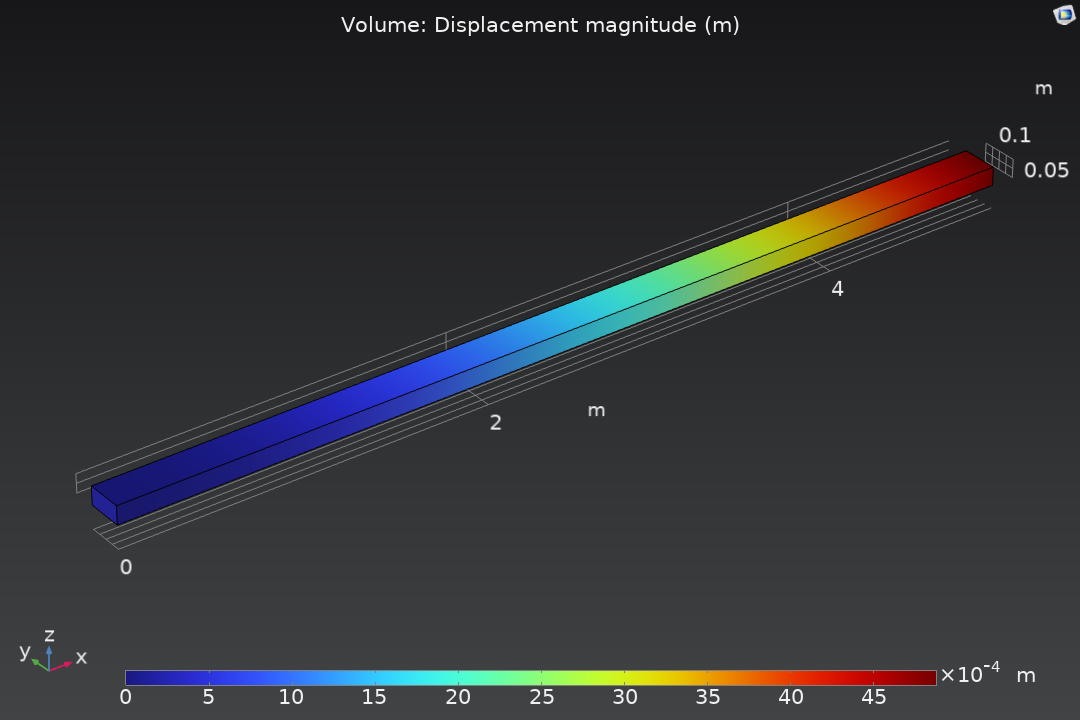
\includegraphics[width=\textwidth]{imgs/hw9/volumedisplacement.png}
        \caption{~}\label{fig9:barSteela}
    \end{subfigure}
    \begin{subfigure}[c]{0.45\textwidth}
        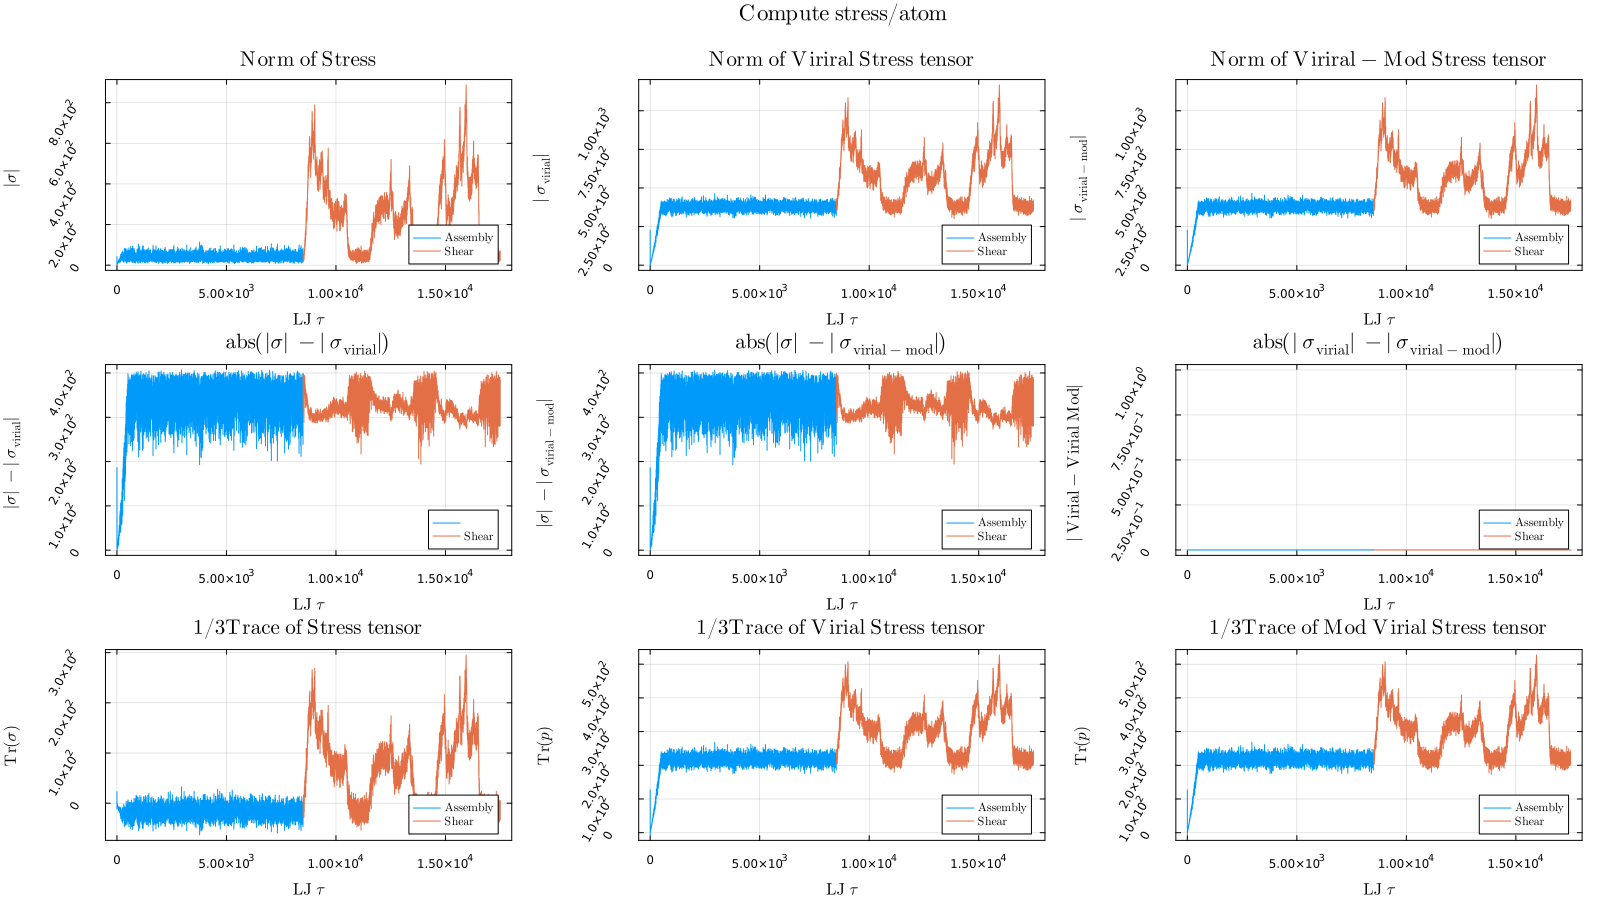
\includegraphics[width=\textwidth]{imgs/hw9/stress.png}
        \caption{~}\label{fig9:barSteelb}
    \end{subfigure}
    \caption{
    Solution of the deformed bar of steel using COMSOL.
    Figure \ref{fig9:barSteela} is the volume displacement magnitude of the bar and in figure \ref{fig9:barSteelb} shows the stress over the bar and the physical displacement.
    }
    \label{fig9:barSteel}
\end{figure}

% https://www.comsol.com/model/channel-beam-8520
% https://www.comsol.com/model/large-deformation-analysis-of-a-beam-204

\end{document}